\documentclass{article}
\usepackage[submission]{colm2026_conference}

\usepackage{microtype}
\usepackage{hyperref}
\usepackage{url}
\usepackage{booktabs}
\usepackage{amsmath}
\usepackage{amssymb}
\usepackage{graphicx}
\usepackage{multirow}
\usepackage{xcolor}
\usepackage{subcaption}
\usepackage{enumitem}
\usepackage{amsthm}
\newtheorem{theorem}{Theorem}

\usepackage{lineno}

\definecolor{darkblue}{rgb}{0, 0, 0.5}
\hypersetup{colorlinks=true, citecolor=darkblue, linkcolor=darkblue, urlcolor=darkblue}

\newcommand{\fix}{\marginpar{FIX}}
\newcommand{\new}{\marginpar{NEW}}

\title{How Reliable Are VLM Judges? Conformal Prediction Reveals \\ Task-Dependent Uncertainty in Multimodal Evaluation}

\author{Anonymous authors\\Paper under double-blind review}

\begin{document}

\ifcolmsubmission
\linenumbers
\fi

\maketitle

\begin{abstract}
As multimodal AI agents are deployed in real-world applications such as navigating web interfaces, interpreting screenshots, and analyzing documents, reliably evaluating their visual reasoning becomes critical. Vision-Language Models (VLMs) are the natural choice for automated evaluation since these tasks require understanding both visual and linguistic content, yet a fundamental question remains: when can we trust a VLM judge's score, and when is it unreliable? We address this through conformal prediction, a distribution-free framework that transforms a VLM judge's single-point score into a prediction interval with provable coverage guarantees, requiring only the judge's score-token log-probabilities with no retraining or assumptions about the error distribution. We conduct the first systematic study of conformal prediction for VLM-as-a-Judge, evaluating 8 conformal methods across 3 VLM judges (LLaVA-Critic-7B, Phi-4-reasoning-15B, Gemini~2.5~Flash) on 2 multimodal benchmarks spanning 14,443 samples and 14 visual task categories. Our analysis reveals that evaluation uncertainty is strongly task-dependent: aesthetics and natural image tasks yield tight intervals covering ${\sim}40\%$ of the score range, while chart reasoning and mathematical figures produce intervals covering ${\sim}70\%$, providing practitioners with the first quantitative reliability map for VLM-based evaluation. We formalize this through a \emph{Ranking-Scoring Gap} diagnostic that identifies a failure mode invisible to standard metrics: on chart understanding, the judge achieves the highest ranking correlation across all 14 task types while producing some of the widest prediction intervals---correctly ordering responses but unable to assign reliable absolute scores. To address the task-dependent uncertainty, we propose Mondrian conformal prediction conditioned on task difficulty, producing 16.6\% narrower intervals for easy tasks while improving coverage for hard tasks. We also find that combining multiple judges' logprobs does not outperform the single best judge, suggesting that logprob quality matters more than quantity. Finally, we show that the same judge and method produce $4.5\times$ narrower intervals on a captioning benchmark with multi-annotator ground truth, demonstrating that interval width is driven primarily by task difficulty and annotation quality rather than the conformal method itself.
\end{abstract}

% ============================================================================
\section{Introduction}
\label{sec:intro}

Large Vision-Language Models (VLMs) are increasingly used as automated judges to evaluate multimodal AI systems~\citep{chen2024mllmasajudge,li2024vlrewardbench}. This \emph{VLM-as-a-Judge} paradigm extends the established LLM-as-a-Judge framework~\citep{zheng2023judging} to tasks requiring visual understanding---evaluating chart comprehension, visual question answering, image captioning, and AI-generated image quality. As multimodal AI agents are deployed in high-stakes applications such as medical image analysis~\citep{chaves2025clinical}, web navigation~\citep{deng2023mind2web}, and document understanding, the reliability of these automated evaluations becomes critical.

However, VLM judges produce only point scores, offering no indication of when their evaluations can be trusted and when they are unreliable. A judge that assigns a score of 4 out of 5 to a visual question answer may be confidently correct or wildly guessing---the user has no way to distinguish these cases. This problem is especially acute in the multimodal setting, where the judge must simultaneously assess textual coherence and visual grounding, introducing uncertainty sources absent in text-only evaluation. Consider the task of evaluating whether an AI assistant correctly described the data trends in a bar chart: the judge must parse the chart visually, extract the relevant data, understand the question, and then assess the answer's accuracy---each step introducing potential error that compounds into evaluation uncertainty.

The scale of this reliability problem is substantial. On the MLLM-as-a-Judge benchmark~\citep{chen2024mllmasajudge}, even the best VLM judges achieve only 32--34\% exact-match accuracy with human annotators on a 5-point Likert scale. While this improves to 70--76\% within $\pm 1$ point, the remaining 24--30\% of evaluations are off by 2 or more points---potentially miscategorizing excellent answers as mediocre or vice versa. Standard metrics like Pearson correlation ($\rho = 0.30$--$0.46$) confirm weak overall alignment. Without uncertainty quantification, practitioners have no way to know which of the judge's evaluations fall into the reliable majority versus the problematic minority.

Conformal prediction~\citep{vovk2005algorithmic} offers a principled solution: given a calibration set with human-annotated ground truth, it transforms the judge's point score into a prediction interval with provable coverage guarantees. If we set the target coverage to $90\%$, the interval is guaranteed to contain the true human score at least $90\%$ of the time, regardless of the judge model's error distribution. Crucially, conformal prediction is \emph{post-hoc}---it requires no retraining of the judge and operates solely on the score-token log-probabilities that VLMs naturally produce during inference. This makes it immediately deployable with any existing VLM judge pipeline.

\citet{sheng2025analyzing} recently demonstrated the effectiveness of conformal prediction for text-only LLM judges on natural language generation tasks, evaluating 9 conformal methods across 3 LLM judges on summarization (SummEval, DialSumm) and reasoning (ROSCOE) benchmarks. They showed that conformal intervals provide coverage guarantees, that boundary adjustment improves calibration for discrete rating scales, and that interval midpoints can serve as calibrated score estimates. We extend this framework to the multimodal setting, where several new challenges arise:

\begin{enumerate}[leftmargin=*,itemsep=2pt,topsep=2pt]
\item \textbf{Cross-modal uncertainty:} VLM judges operate over both visual and textual modalities, potentially compounding uncertainty from visual perception errors and language understanding errors.
\item \textbf{Discrete ground truth:} Multimodal evaluation benchmarks often use single-annotator integer ground truth rather than averaged continuous scores, requiring careful handling of discreteness through boundary adjustment.
\item \textbf{Task diversity:} The diversity of visual task types---from aesthetics assessment to mathematical reasoning to chart understanding---introduces systematic variation in judge reliability that has no direct analogue in text-only evaluation where tasks (summarization, dialogue) are more homogeneous.
\item \textbf{Model access:} The emerging ecosystem of VLM judges spans open-source models with full logprob access (LLaVA-Critic, Phi-4) and closed-source API models with limited logprob access (Gemini), requiring methods that work across access levels.
\end{enumerate}

Our study makes the following contributions:

\begin{itemize}[leftmargin=*,itemsep=2pt,topsep=2pt]
\item We present the \textbf{first systematic study of conformal prediction for VLM-as-a-Judge}, evaluating 8 conformal methods across 3 VLM judges of varying architecture and scale (7B open-source, 15B reasoning model, and closed-source API) on 14,443 multimodal evaluation instances across 2 benchmarks.

\item We reveal that \textbf{evaluation uncertainty is strongly task-dependent}: prediction interval width varies by up to 70\% across 14 visual task categories, with Vision-Heavy tasks (math, charts, infographics) producing intervals averaging 3.21 on a 4-point range versus 2.59 for Knowledge/Web tasks. This provides practitioners with the first quantitative reliability map for VLM-based evaluation.

\item We uncover a \textbf{ranking-scoring decoupling} invisible to standard metrics: judges can achieve high ranking correlation (e.g., Pearson $= 0.507$ on ChartQA) while simultaneously producing wide prediction intervals (width $= 3.08$), meaning they correctly order responses but cannot assign reliable absolute scores. This has direct implications for choosing between pairwise comparison and Likert-scale scoring protocols.

\item We demonstrate that \textbf{interval width is driven by task difficulty and annotation quality}, not the conformal method: the same judge and method produce $4.5\times$ narrower intervals (0.68 vs.\ 3.05) on a captioning benchmark with multi-annotator ground truth compared to a VQA benchmark with single-annotator labels.

\item We propose \textbf{Mondrian conformal prediction} conditioned on task difficulty, which yields 16.6\% narrower intervals for easy tasks while simultaneously improving coverage for hard tasks---the first application of task-conditional CP to VLM judge evaluation.

\item We introduce a \textbf{CP-Reliability Diagnostic} based on the \emph{Ranking-Scoring Gap}, a metric that formalizes the decoupling between ranking quality and scoring precision, and show that \textbf{multi-judge feature fusion does not outperform the single best judge} (a negative but informative result for practitioners).
\end{itemize}

% ============================================================================
\section{Related work}
\label{sec:related}

\paragraph{LLM-as-a-Judge.}
Using LLMs as automated evaluators has become the dominant paradigm for evaluating natural language generation~\citep{zheng2023judging,liu2023geval}. G-Eval~\citep{liu2023geval} uses GPT-4 with chain-of-thought prompting to score text quality, demonstrating higher correlation with human judgments than traditional metrics like ROUGE and BERTScore. The MT-Bench and Chatbot Arena frameworks~\citep{zheng2023judging} establish LLM-as-a-Judge for pairwise preference evaluation, revealing systematic biases including position bias, self-enhancement bias, and verbosity bias. SocREval~\citep{he2024soceval} designs prompts specifically for reasoning evaluation. These works establish the paradigm but focus exclusively on text-only tasks and point-score evaluation without uncertainty quantification.

\paragraph{VLM-as-a-Judge.}
Recent work extends LLM-as-a-Judge to multimodal evaluation. \citet{chen2024mllmasajudge} introduce the MLLM-as-a-Judge benchmark, evaluating VLM judges (GPT-4V, Gemini, CogVLM, LLaVA) across 14 visual task categories and finding that GPT-4V achieves the highest alignment with human judgments (42\% exact accuracy). LLaVA-Critic~\citep{xiong2024llavacritic} trains a specialized VLM judge for multimodal evaluation, while VL-RewardBench~\citep{li2024vlrewardbench} provides a reward benchmark finding that $>67\%$ of VLM judge errors are perceptual rather than reasoning-based. Despite growing adoption, VLM judge reliability remains poorly understood---existing benchmarks report aggregate accuracy metrics but provide no per-instance uncertainty estimates.

\paragraph{Uncertainty quantification for LLM judges.}
Quantifying the uncertainty of LLM-as-a-Judge evaluations is an emerging and important area. \citet{wagner2024llmconfidence} propose black-box uncertainty quantification for LLM judges using token-level probabilities, finding that judge confidence does not always correlate with accuracy. Other approaches include prompting LLMs to self-report confidence~\citep{xiong2024selfconsistency}, which can suffer from overconfidence, and consistency-based approaches that require multiple generations~\citep{tian2023consistency}. Most relevant to our work, \citet{sheng2025analyzing} apply conformal prediction to LLM judges on text-only tasks, evaluating 9 methods across summarization, dialogue, and reasoning benchmarks with 3 LLM judges (GPT-4o mini, DeepSeek-R1-32B, Qwen2.5-72B). They demonstrate that conformal intervals provide coverage guarantees, that boundary adjustment improves calibration for discrete rating scales, and that R2CCP achieves the best coverage-width tradeoff. Our work extends this framework to VLM judges, revealing multimodal-specific phenomena---task-dependent uncertainty and ranking-scoring decoupling---that have no analogue in their text-only analysis.

\paragraph{Conformal prediction for language models.}
Conformal prediction~\citep{vovk2005algorithmic} has drawn increasing interest for uncertainty quantification in LLMs~\citep{campos2024conformal} due to its distribution-free and post-hoc nature with provable statistical guarantees. Recent works apply conformal prediction primarily to classification tasks: multiple-choice QA~\citep{kumar2023conformal,su2024api}, factual consistency~\citep{quach2024conformal,mohri2024language}, and calibrated risk control~\citep{angelopoulos2022conformal}. These studies typically focus on ensuring the correct answer is included in an unordered prediction set. In contrast, we focus on \emph{regression-based} conformal prediction for rating tasks, constructing continuous prediction intervals that reflect the variability of human judgments---a setting with ordinal preference structure that differs fundamentally from classification. We additionally explore \emph{Mondrian} conformal prediction~\citep{vovk2005algorithmic}, which computes group-conditional quantiles, enabling task-adapted intervals that are tighter for easy tasks and more conservative for hard tasks.

% ============================================================================
\section{Background}
\label{sec:background}

\subsection{VLM-as-a-Judge framework}
\label{sec:vlm_judge}

In the VLM-as-a-Judge framework, a vision-language model $M$ is used to evaluate the quality of a response to a visually-grounded question. Given an image $I$, a question $q$, and a candidate answer $a$, the judge is prompted with a chain-of-thought evaluation instruction and produces a response containing a score $y_0$ on a discrete Likert scale $\{1, 2, \ldots, K\}$ (we use $K=5$):
\begin{equation}
M(I, q, a) = (z, y_0),
\end{equation}
where $z$ denotes the token logits at the score position. The judge first analyzes the image and evaluates the response (the chain-of-thought reasoning), then outputs a final score. We extract the log-probabilities for each rating token $k \in \{1, \ldots, K\}$ at the score position, yielding a $K$-dimensional feature vector:
\begin{equation}
\mathbf{x} = [\log P(\text{``1''}), \log P(\text{``2''}), \ldots, \log P(\text{``$K$''})].
\label{eq:features}
\end{equation}
This feature vector captures the judge's distributional belief over possible scores---a concentrated distribution (one score with high probability) indicates high confidence, while a spread distribution indicates uncertainty. We refer to this as the \emph{Signal 2} (S2) feature following the nomenclature established in our pipeline. Early experiments with additional features---actor-model generation entropy (Signal 1) and derived statistics of the score distribution like entropy and margin (Signal 3)---showed no improvement over S2 alone, as S3 is a deterministic function of S2 and S1 requires separate actor-model ground truth. We therefore use S2 exclusively.

\subsection{Conformal prediction}
\label{sec:cp}

Conformal prediction~\citep{vovk2005algorithmic} is a distribution-free framework for constructing prediction intervals with coverage guarantees. Given a calibration set $\{(\mathbf{x}_i, y_i)\}_{i=1}^{n}$ where $\mathbf{x}_i$ is the feature vector and $y_i$ is the human ground truth score, and a nonconformity score function $s(\mathbf{x}, y)$ that measures how ``unusual'' a prediction is relative to the ground truth, the method constructs intervals as follows.

For regression tasks, a common nonconformity score is the absolute residual $s(\mathbf{x}, y) = |\hat{y} - y|$, where $\hat{y} = f(\mathbf{x})$ is a point prediction from a model trained on the calibration set. Given a user-specified miscoverage rate $\alpha$, we compute the $\lceil (n+1)(1-\alpha) \rceil / n$ quantile $\hat{q}$ of the calibration nonconformity scores, then construct the prediction interval for a test point $\mathbf{x}_\text{test}$:
\begin{equation}
\mathcal{C}(\mathbf{x}_\text{test}) = [\hat{y}_\text{test} - \hat{q},\ \hat{y}_\text{test} + \hat{q}].
\end{equation}
This interval satisfies the marginal coverage guarantee~\citep{angelopoulos2023gentle}:
\begin{equation}
1 - \alpha \leq \mathbb{P}(y_\text{test} \in \mathcal{C}(\mathbf{x}_\text{test})) \leq 1 - \alpha + \frac{1}{n+1},
\label{eq:coverage}
\end{equation}
assuming the calibration and test data are exchangeable (i.e., the joint distribution remains the same after any permutations on these two sets).

Two notable advantages of conformal prediction make it particularly suitable for VLM judge calibration. First, it is \emph{post-hoc}---it does not require retraining or fine-tuning the judge model, operating solely on the logprob features extracted from a single evaluation run. Second, it is \emph{distribution-free}---no assumptions about the judge's error distribution are needed, which is important since VLM judge errors are highly heteroscedastic across task types.

\subsection{Conformal prediction methods}
\label{sec:cp_methods}

We evaluate 8 conformal prediction methods spanning regression-based and classification-based approaches, following the comprehensive evaluation of \citet{sheng2025analyzing}.

\paragraph{Regression-based methods.} These methods construct continuous prediction intervals using the logit features directly:
\begin{itemize}[leftmargin=*,itemsep=1pt,topsep=2pt]
\item \textbf{Naive Split Conformal Prediction:} The simplest baseline---fits a point predictor on the calibration set and uses absolute residuals as nonconformity scores.
\item \textbf{Conformalized Quantile Regression (CQR;~\citealp{romano2019conformalized}):} Fits conditional quantile regressors for the $\alpha/2$ and $1-\alpha/2$ quantiles, then applies conformal correction. Produces asymmetric intervals adapted to the local data density.
\item \textbf{Asymmetric CQR~\citep{sesia2020comparison}:} A variant of CQR that separately calibrates upper and lower bounds.
\item \textbf{Conformal Histogram Regression (CHR;~\citealp{sesia2021conformal}):} Uses a histogram-based quantile estimator, producing intervals adapted to the conditional distribution of scores.
\item \textbf{Locally-adaptive Variance-based Distribution-free prediction (LVD;~\citealp{lin2021locally}):} Uses kernel regression-based quantile estimation for locally adaptive intervals.
\item \textbf{Boosted CQR and Boosted LCP~\citep{xie2024boosted}:} Boosted variants that iteratively refine the quantile estimates for improved conditional coverage.
\item \textbf{R2CCP~\citep{guha2024conformal}:} Models the conditional distribution directly via a neural network with softmax output (Regression-as-Classification for Conformal Prediction). Particularly well-suited to settings where features are weak predictors, as it learns a full distribution rather than quantile estimates.
\end{itemize}

\paragraph{Classification-based methods.} These methods treat rating-based evaluation as an ordinal classification problem:
\begin{itemize}[leftmargin=*,itemsep=1pt,topsep=2pt]
\item \textbf{Ordinal Adaptive Prediction Sets (OrdinalAPS;~\citealp{lu2022fair}):} Extends adaptive prediction sets to the ordinal setting, constructing contiguous prediction sets that respect the ordinal structure of ratings.
\end{itemize}

Note that we also attempted Ordinal Risk Control (OrdinalRC) but encountered import compatibility issues with our software environment. Following \citet{sheng2025analyzing}, classification-based methods use token probabilities (softmax of logits) as input rather than raw logits, since probabilities serve as natural class probability estimates.

\subsection{Boundary adjustment for discrete scales}
\label{sec:boundary}

A key challenge in applying conformal prediction to VLM judges is that ground truth scores are discrete integers while prediction intervals are continuous. Following \citet{sheng2025analyzing}, we apply boundary adjustment to align continuous prediction intervals with the discrete rating scale. The nonconformity score is modified as:
\begin{equation}
s'(\mathbf{x}, y) = \begin{cases}
s(\mathbf{x}, \lceil y \rceil) & \text{if } y \leq \lfloor \hat{y} \rfloor, \\
s(\mathbf{x}, y) & \text{otherwise,} \\
s(\mathbf{x}, \lfloor y \rfloor) & \text{if } y \geq \lceil \hat{y} \rceil,
\end{cases}
\end{equation}
which transforms the continuous interval $[l, u]$ to the ordinal interval $[\lceil l \rceil, \lfloor u \rfloor]$, ensuring endpoints align with valid rating labels. \citet{sheng2025analyzing} prove that this adjustment is non-decreasing in coverage:

\begin{theorem}[Non-decreasing Coverage After Boundary Adjustment, \citealp{sheng2025analyzing}]
If the adjustment shrinks the interval (i.e., $l' = \lceil l \rceil$, $u' = \lfloor u \rfloor$), coverage is preserved: $\mathbb{P}(y_\text{test} \in \mathcal{C}'(\mathbf{x}_\text{test})) \geq 1 - \alpha$. If at least one boundary is expanded (i.e., $l' = \lfloor l \rfloor$ or $u' = \lceil u \rceil$), coverage increases: $\mathbb{P}(y_\text{test} \in \mathcal{C}'(\mathbf{x}_\text{test})) > 1 - \alpha$.
\end{theorem}

This property is especially important in our setting because our ground truth uses only 5 discrete integer values (compared to 13 fractional values in SummEval from averaging 3 annotators), making boundary adjustment substantially more impactful.

\subsection{Mondrian conformal prediction}
\label{sec:mondrian}

Standard conformal prediction computes a single quantile $\hat{q}$ from the entire calibration set, producing intervals that are exchangeable across all test samples. However, our per-dataset analysis (\S\ref{sec:task_dependent}) reveals that VLM judge uncertainty varies dramatically across visual task types. Mondrian conformal prediction~\citep{vovk2005algorithmic} addresses this by partitioning the data into groups and computing separate quantiles per group, providing group-conditional coverage guarantees.

We partition the 14 datasets into three difficulty groups based on their per-dataset R2CCP width from an initial standard CP run:
\begin{itemize}[leftmargin=*,itemsep=1pt,topsep=2pt]
\item \textbf{Easy} (width $<$ 2.5): AesBench, MM-Vet, WIT, COCO --- tasks where the judge is relatively well-calibrated.
\item \textbf{Medium} (width 2.5--3.2): Mind2Web, Conceptual Captions, TextVQA, LLaVA-Bench, VisitBench, ChartQA --- moderate difficulty tasks.
\item \textbf{Hard} (width $>$ 3.2): ScienceQA, MathVista, DiffusionDB, InfographicsVQA --- tasks where the judge struggles most.
\end{itemize}

By computing separate conformal quantiles per group, Mondrian CP can assign tighter intervals to easy tasks (where the judge's nonconformity scores are concentrated near zero) without sacrificing coverage on hard tasks (where larger intervals are genuinely needed). The coverage guarantee becomes group-conditional: $\mathbb{P}(y_\text{test} \in \mathcal{C}(\mathbf{x}_\text{test}) \mid G = g) \geq 1 - \alpha$ for each group $g$.

\subsection{CP-Reliability Diagnostic: the Ranking-Scoring Gap}
\label{sec:rsg}

Standard evaluation metrics for VLM judges (Pearson correlation, accuracy, MAE) capture either ranking quality or scoring precision, but not the relationship between them. Our analysis reveals cases where these diverge: a judge may rank responses correctly (high Pearson) while producing unreliable absolute scores (wide CP intervals). To formalize this, we introduce the \emph{Ranking-Scoring Gap} (RSG):

\begin{equation}
\text{RSG}(d) = |\rho_d| - \text{CP-Info}(d), \quad \text{where} \quad \text{CP-Info}(d) = 1 - \frac{w_d}{K - 1},
\label{eq:rsg}
\end{equation}

where $\rho_d$ is the Pearson correlation for dataset $d$, $w_d$ is the R2CCP interval width, and $K - 1 = 4$ is the score range. CP-Informativeness ranges from 0 (full-range, uninformative intervals) to 1 (zero-width, perfectly informative intervals).

A \textbf{high positive RSG} indicates that the judge ranks well but produces wide (uninformative) intervals---the judge's ranking ability exceeds its scoring precision. A \textbf{negative RSG} indicates the opposite: intervals are more informative than the ranking correlation would suggest. The RSG provides practitioners with a single diagnostic that identifies tasks where pairwise comparison should be preferred over Likert scoring.

\subsection{Midpoint as calibrated score}
\label{sec:midpoint_background}

\citet{sheng2025analyzing} propose using the midpoint of the prediction interval as a calibrated score estimate: $\hat{y}_\text{mid} = (l + u) / 2$. The intuition is that the midpoint is evaluated in a shorter interval rather than the entire rating range, potentially providing a less biased estimate. They demonstrate that midpoints outperform raw judge scores on MSE and MAE in text-only settings. We evaluate whether this finding transfers to VLM judges.

% ============================================================================
\section{Experimental setup}
\label{sec:setup}

\subsection{Datasets}
\label{sec:datasets}

We use two multimodal evaluation benchmarks with human-annotated ground truth scores, chosen to span different task complexities and annotation qualities.

\paragraph{MLLM-as-a-Judge~\citep{chen2024mllmasajudge}.} This comprehensive benchmark contains 5,717 evaluation instances spanning 14 visual task categories. Each instance consists of an image, a question, an AI-generated answer (from one of 5 models: GPT-4V, Gemini, CogVLM, LLaVA, or a reference answer), and a human-annotated quality score on a 1--5 integer Likert scale from a single annotator. The 14 datasets are grouped into 4 meta-categories:

\begin{itemize}[leftmargin=*,itemsep=1pt,topsep=2pt]
\item \textbf{Vision-Heavy} (2,383 samples): MathVista (790), ChartQA (400), InfographicsVQA (398), ScienceQA (396), TextVQA (399)---tasks requiring deep visual parsing of structured visual content like mathematical figures, charts, infographics, scientific diagrams, and text in images.
\item \textbf{General VQA} (1,448 samples): COCO (397), MM-Vet (258), LLaVA-Bench (396), VisitBench (397)---general visual question answering about natural images.
\item \textbf{Knowledge/Web} (1,195 samples): WIT (399), Mind2Web (398), Conceptual Captions (398)---tasks involving web content, knowledge retrieval, and web navigation screenshots.
\item \textbf{Aesthetics/AI} (691 samples): AesBench (392), DiffusionDB (299)---aesthetics assessment and AI-generated image evaluation.
\end{itemize}

The score distribution is skewed toward higher scores: GT$=$4 comprises 31.3\% of samples, GT$=$5 comprises 23.0\%, while GT$=$1 and GT$=$2 together comprise only 23.6\%. This imbalance is important because it affects both judge bias patterns and conditional coverage.

\paragraph{Polaris~\citep{wada2024polos}.} This captioning benchmark contains 8,726 image-caption pairs with ground truth quality scores derived from 3 or more human annotators, averaged to produce continuous scores on a 0--1 scale (linearly mapped to 1--5 for our experiments). The Polaris dataset provides a complementary evaluation setting that differs from MLLM-Judge in three key ways: (1) it involves a single, well-defined task (caption quality assessment) rather than 14 diverse task types; (2) ground truth is averaged from multiple annotators, substantially reducing annotation noise; and (3) the task is more constrained---evaluating whether a caption describes an image, rather than open-ended VQA requiring reasoning. This enables us to isolate the effect of task difficulty and annotation quality on conformal interval width.

\subsection{VLM judges}
\label{sec:judges}

We evaluate three VLM judges spanning different architectures, scales, access levels, and design philosophies, providing a diverse testbed for conformal prediction:

\paragraph{LLaVA-Critic-7B~\citep{xiong2024llavacritic}.} An open-source 7B-parameter model based on the LLaVA-NeXT architecture with a Qwen-2 language backbone, specifically trained for multimodal evaluation tasks. We use SDPA attention (critical for correct sliding window attention behavior) and chain-of-thought prompting adapted from the MLLM-as-a-Judge benchmark, instructing the judge to first analyze the image, then evaluate the response, and finally provide a score (Appendix~\ref{app:prompts}). This model represents the class of small, specialized evaluation models. It produces the most calibrated score distributions among our judges, with only 25.6\% of samples having maximum softmax probability $> 0.99$.

\paragraph{Phi-4-reasoning-vision-15B~\citep{abdin2025phi4reasoning}.} An open-source 15B-parameter reasoning model from Microsoft that uses an explicit $\langle\text{think}\rangle$ mode for extended chain-of-thought reasoning before producing a final answer. When given the evaluation prompt, Phi-4 generates 300--1,100 reasoning tokens before scoring, producing detailed step-by-step evaluation. This model provides several contrasts to LLaVA-Critic: it is twice as large (15B vs.\ 7B), uses structured reasoning (explicit think mode), but produces more peaked score distributions (43\% of samples $> 0.99$). Despite its reasoning capability, it exhibits a strong ``gravity toward 4'' effect where 56\% of GT$=$4 and 57\% of GT$=$5 predictions land on score 4. We use a separate conda environment with transformers$\geq$4.57.1 (required for Phi-4's Siglip2VisionModel).

\paragraph{Gemini 2.5 Flash~\citep{google2025gemini25}.} A closed-source commercial model accessed via the Google Vertex AI API with top-20 log-probability support (not available through Google AI Studio). As the largest-scale model in our evaluation, Gemini represents the frontier of commercial VLM judges. It achieves the highest ranking correlation (Pearson $= 0.459$) but produces the most overconfident score distributions (83\% of samples $> 0.99$, 77\% $> 0.999$). The near-zero overall bias ($-0.045$) makes it the most balanced scorer, though it makes larger absolute errors when wrong ($\pm 1$ accuracy of 70.3\% vs.\ 75--76\% for open-source judges). API cost for the full dataset was approximately \$2--3.

All three judges use the same chain-of-thought evaluation prompt on MLLM-as-a-Judge (Appendix~\ref{app:prompts}). For Polaris, we adapt the prompt for caption evaluation. The diversity of judges---open-source specialized (LLaVA-Critic), open-source reasoning (Phi-4), closed-source commercial (Gemini)---enables us to assess whether conformal prediction findings generalize across model architectures and access patterns.

\subsection{Feature extraction}
\label{sec:features}

For each evaluation instance, we extract the judge's score-token log-probabilities as described in Equation~\ref{eq:features}. The extraction process requires locating the score token within the judge's generated output, which is non-trivial because chain-of-thought reasoning produces lengthy outputs containing many digit tokens (e.g., ``the response covers 3 of 5 key points'') before the final score.

We employ a three-strategy approach to locate the score token: (1) search for a ``Score:'' prefix followed by a digit token, (2) search for other score keywords (``rating'', ``score'') followed by a digit, (3) scan backwards from the end of the generated sequence to find the last digit token ``1'' through ``5''. The backwards scan is critical---forward scanning would incorrectly identify digits in the reasoning chain rather than the final score.

At the identified score position, we extract the log-probabilities for all 5 rating tokens (``1'' through ``5''). For open-source models, we access the full logit distribution from the model's generation output. For Gemini via Vertex AI, we request top-20 log-probabilities, which is sufficient since rating tokens are almost always within the top-20 at the score position. If a rating token is not present in the available log-probabilities, we assign a default value of $\log(10^{-5}) \approx -11.5$. This yields a 5-dimensional feature vector per sample.

\paragraph{Chain-of-thought prompting.} We use chain-of-thought prompting following the evaluation protocol of \citet{chen2024mllmasajudge}. The prompt instructs the judge to: (1) examine the image attentively, (2) conduct a comprehensive analysis, (3) critically evaluate the response, and (4) provide a final score on a 1--5 scale with a detailed rubric. Compared to a generic scoring prompt without chain-of-thought, CoT prompting improves Pearson correlation from 0.380 to 0.402 (+5.8\%), Spearman from 0.314 to 0.356 (+13.4\%), and---critically for conformal prediction---reduces the fraction of overconfident predictions (softmax max $> 0.99$) from 51.4\% to 25.6\% (-50\%). The reduction in overconfidence gives conformal prediction methods more distributional signal to work with.

\subsection{Evaluation protocol}
\label{sec:protocol}

Following \citet{sheng2025analyzing}, we randomly split each dataset 50/50 into calibration and test sets across 10 random seeds (seeds 1--10) and report mean $\pm$ standard deviation. We use significance level $\alpha = 0.10$, targeting 90\% coverage. The 50/50 split provides approximately 2,859 calibration and 2,858 test samples per seed for MLLM-Judge, and 4,363/4,363 for Polaris. We report:

\begin{itemize}[leftmargin=*,itemsep=1pt,topsep=2pt]
\item \textbf{Coverage:} the fraction of test samples where the ground truth falls within the prediction interval. Target: $\geq 0.90$.
\item \textbf{Width:} the average prediction interval width on the 1--5 scale (range: 0 to 4). Lower is better given sufficient coverage.
\item \textbf{Point prediction metrics:} Pearson $\rho$, Spearman $\rho_s$, and Kendall $\tau$ correlations; exact-match accuracy; relaxed $\pm 1$ accuracy; mean absolute error (MAE).
\item \textbf{Judge bias:} mean signed error (judge score $-$ human GT), stratified by GT score level.
\end{itemize}

Both raw (continuous) and boundary-adjusted (discrete) intervals are reported for all methods. For per-dataset analyses, we run R2CCP independently on each of the 14 datasets to assess conditional coverage and task-dependent interval widths.

% ============================================================================
\section{Results}
\label{sec:results}

\subsection{Point prediction performance}
\label{sec:point_prediction}

Before examining conformal prediction, we establish baseline point prediction performance for all three judges on MLLM-as-a-Judge (Table~\ref{tab:cross_judge}).

All three judges achieve comparable exact accuracy (32--34\%) but differ substantially in other metrics. Gemini achieves the highest correlation (Pearson $= 0.459$), Phi-4 the lowest MAE (1.005) and lowest bias ($+0.08$), and LLaVA-Critic the best-calibrated logprob distributions (25.6\% overconfident). These differences have important implications for conformal prediction, as we discuss in \S\ref{sec:cross_judge}.

\paragraph{Error distribution.} Across all judges, approximately 32--34\% of predictions exactly match human ground truth, and 70--76\% fall within $\pm 1$ point. The remaining 24--30\% are off by $\geq 2$ points, representing potentially consequential evaluation errors. The 3-class accuracy (merging scores into Bad$=\{1\}$, Medium$=\{2,3\}$, Good$=\{4,5\}$) reaches 58\%, suggesting that judges capture broad quality categories better than fine-grained distinctions.

\paragraph{Judge bias.} All three judges exhibit positive bias---they systematically overscore bad answers and underscore excellent ones. For GT$=$1 (worst quality), the mean bias ranges from $+0.89$ (Gemini) to $+1.98$ (Phi-4), meaning judges assign an average score of 2.9--3.0 to answers that humans rate as 1. For GT$=$5 (best quality), bias is negative ($-0.74$ to $-1.04$), indicating underscoring. Gemini is the most balanced overall ($-0.045$ mean bias), while LLaVA-Critic shows moderate positive bias ($+0.38$) and Phi-4 exhibits the ``gravity toward 4'' phenomenon with near-zero overall bias ($+0.08$) but extreme compression toward score 4.

\paragraph{Comparison with existing judges in the MLLM-Judge benchmark.} Our LLaVA-Critic-7B with CoT prompting achieves 75.1\% $\pm 1$ accuracy, placing it between GPT-4V (82.6\%) and the original LLaVA (72.5\%) in the benchmark's judge comparison. This is competitive given that LLaVA-Critic is a 7B model compared to GPT-4V. More importantly for our purposes, the error patterns are consistent across all judges---all show positive bias and similar error distributions---suggesting that our conformal prediction findings generalize beyond specific judge models.

\subsection{Conformal methods comparison}
\label{sec:methods_comparison}

Table~\ref{tab:all_methods} presents the coverage and width for all 8 conformal prediction methods on the MLLM-as-a-Judge benchmark using LLaVA-Critic-7B. The methods fall into three performance tiers.

\begin{table}[t]
\centering
\caption{Conformal prediction methods on MLLM-as-a-Judge (LLaVA-Critic-7B, $\alpha=0.10$, 10 seeds). Methods grouped by performance tier. Bold indicates best within well-calibrated methods.}
\label{tab:all_methods}
\small
\begin{tabular}{lcccc}
\toprule
\textbf{Method} & \textbf{Cov. (raw)} & \textbf{Width (raw)} & \textbf{Cov. (adj.)} & \textbf{Width (adj.)} \\
\midrule
\multicolumn{5}{l}{\emph{Tier 1: Well-calibrated (coverage $\approx$ 90\%, informative width)}} \\
\textbf{R2CCP} & \textbf{.900$\pm$.016} & 3.05$\pm$.10 & .981$\pm$.005 & 3.60$\pm$.09 \\
CHR & .880$\pm$.010 & \textbf{2.97$\pm$.07} & .965$\pm$.006 & \textbf{3.43$\pm$.10} \\
Boosted LCP & .863$\pm$.012 & 3.02$\pm$.03 & .977$\pm$.004 & 3.51$\pm$.04 \\
\midrule
\multicolumn{5}{l}{\emph{Tier 2: Moderate (slight over/under-coverage, moderate width)}} \\
Naive Split CP & .895$\pm$.009 & 3.23$\pm$.06 & .990$\pm$.003 & 3.78$\pm$.04 \\
LVD & .894$\pm$.009 & 3.21$\pm$.11 & .988$\pm$.005 & 3.71$\pm$.11 \\
Boosted CQR & .878$\pm$.009 & 3.54$\pm$.09 & .997$\pm$.002 & 3.93$\pm$.04 \\
\midrule
\multicolumn{5}{l}{\emph{Tier 3: Degenerate (massive over-coverage, uninformative)}} \\
CQR & .996$\pm$.005 & 3.95$\pm$.06 & 1.00$\pm$.000 & 4.00$\pm$.00 \\
Asym. CQR & .996$\pm$.005 & 3.95$\pm$.06 & 1.00$\pm$.000 & 4.00$\pm$.00 \\
OrdinalAPS & .999$\pm$.000 & 3.99$\pm$.00 & .999$\pm$.000 & 3.99$\pm$.00 \\
\bottomrule
\end{tabular}
\end{table}

\paragraph{Tier 1: Well-calibrated methods.} R2CCP achieves exactly 90.0\% raw coverage---the closest to the 90\% target---with width 3.05. CHR produces the narrowest raw intervals (2.97) but slightly under-covers (88.0\%). Boosted LCP achieves the most stable intervals (lowest width std of 0.03) but under-covers at 86.3\%. After boundary adjustment, all Tier 1 methods exceed 96\% coverage.

\paragraph{Tier 3: Degenerate methods.} CQR, Asymmetric CQR, and OrdinalAPS are effectively unusable in our setting. They over-cover to ${\sim}100\%$ with near-full-range intervals (${\sim}4.0$ on a 1--5 scale). After boundary adjustment, CQR/AsymCQR produce intervals of exactly $[1, 5]$ for every sample, providing zero discrimination.

\paragraph{Why CQR fails but R2CCP succeeds.} This failure is not a bug but a consequence of weak features. CQR's base quantile regressor (GradientBoosting) estimates the $\alpha/2$ and $1-\alpha/2$ conditional quantiles from the 5-dimensional logprob features. When features are weak predictors (Pearson $= 0.40$), the estimated quantiles span nearly the full $[1, 5]$ range for every sample, producing uniformly wide intervals. The conformal correction can only widen, never narrow, these intervals. R2CCP succeeds because it takes a fundamentally different approach: it models the conditional distribution $P(y|\mathbf{x})$ directly via a neural network with softmax output, discretizing the target into bins and learning a full distributional mapping. This regression-as-classification approach is better suited to weak-signal settings where learning quantile boundaries is difficult but learning distributional shifts is feasible.

\paragraph{Recommendation.} Based on our results, we recommend \textbf{R2CCP} as the default method for VLM judge calibration due to its exact coverage and reasonable width. CHR is preferred when narrower intervals are desired and slight under-coverage is acceptable. We use R2CCP for all subsequent analyses unless stated otherwise.

\subsection{Cross-judge comparison}
\label{sec:cross_judge}

Table~\ref{tab:cross_judge} compares the three VLM judges on both point prediction metrics and conformal prediction intervals. Several non-obvious and practically important patterns emerge.

\begin{table}[t]
\centering
\caption{Cross-judge comparison on MLLM-as-a-Judge (R2CCP, $\alpha=0.10$, 10 seeds). Gemini achieves the narrowest intervals despite the most overconfident logprob distributions.}
\label{tab:cross_judge}
\small
\begin{tabular}{lccc}
\toprule
& \textbf{LLaVA-Critic} & \textbf{Phi-4} & \textbf{Gemini 2.5} \\
& \textbf{7B} & \textbf{15B} & \textbf{Flash} \\
\midrule
\multicolumn{4}{l}{\emph{Point prediction}} \\
Pearson $\rho$ & .402 & .303 & \textbf{.459} \\
Spearman $\rho_s$ & .356 & .293 & \textbf{.446} \\
Kendall $\tau$ & .300 & .251 & \textbf{.377} \\
Accuracy & 32.2\% & \textbf{34.2\%} & 32.1\% \\
$\pm 1$ Accuracy & 75.1\% & \textbf{76.1\%} & 70.3\% \\
MAE & 1.031 & \textbf{1.005} & 1.122 \\
Judge bias & $+0.38$ & $+0.08$ & $\mathbf{-0.05}$ \\
\midrule
\multicolumn{4}{l}{\emph{Score distribution calibration}} \\
Overconf. ($>$0.99) & \textbf{25.6\%} & 43.0\% & 83.0\% \\
Overconf. ($>$0.999) & \textbf{6.6\%} & 16.9\% & 77.4\% \\
\midrule
\multicolumn{4}{l}{\emph{Conformal prediction (R2CCP)}} \\
Coverage (raw) & \textbf{.900} & .891 & .898 \\
Width (raw) & 3.05 & 3.13 & \textbf{2.85} \\
Coverage (adj.) & .981 & .981 & .980 \\
Width (adj.) & 3.60 & 3.70 & \textbf{3.41} \\
\midrule
\multicolumn{4}{l}{\emph{Conformal prediction (CHR)}} \\
Coverage (raw) & .880 & .896 & .880 \\
Width (raw) & 2.97 & 3.16 & \textbf{2.80} \\
\bottomrule
\end{tabular}
\end{table}

\paragraph{The Gemini paradox: overconfidence does not imply poor calibration.} Despite producing the most overconfident score distributions (83\% of softmax maxima $> 0.99$, 77\% $> 0.999$), Gemini yields the \emph{narrowest} conformal intervals (2.85 raw, 3.41 adjusted)---7\% narrower than LLaVA-Critic (3.05 raw) and 9\% narrower than Phi-4 (3.13 raw). This paradox is resolved by understanding what R2CCP uses: it learns a neural network mapping from the 5-dimensional logprob vector to nonconformity scores. Even though Gemini's logprobs are extremely peaked, the relative magnitudes of the 5 log-probabilities still carry discriminative signal (Gemini's Pearson $= 0.459$ is the highest among all judges). R2CCP can exploit this signal even when the distributions appear ``overconfident'' by standard measures. \textbf{This finding has an important practical implication: overconfidence in raw logprob distributions does not imply poor conformal calibration.} The quality of conformal intervals depends on the \emph{signal-to-noise ratio} in the features, not on the \emph{calibration} of the softmax distribution.

\paragraph{Accuracy vs.\ correlation tradeoff.} The three judges reveal a clear tradeoff between accuracy-type metrics and correlation-type metrics. Phi-4 achieves the highest exact accuracy (34.2\%) and lowest MAE (1.005) but the lowest Pearson correlation (0.303). Gemini achieves the highest correlation (0.459) but the lowest $\pm 1$ accuracy (70.3\%) and highest MAE (1.122). This divergence indicates that accuracy and correlation capture fundamentally different aspects of judge quality: correlation measures \emph{ranking ability} (whether the judge correctly orders samples from low to high quality) while accuracy measures \emph{absolute scoring precision} (whether the judge assigns the correct score value). Gemini is the best ranker but makes larger absolute errors when wrong. This distinction becomes central to our ranking-scoring decoupling analysis (\S\ref{sec:decoupling}).

\paragraph{All judges share a positive bias toward overscoring.} All three judges systematically overscore bad answers and underscore excellent ones, though the magnitude varies. Table~\ref{tab:bias} presents the full bias analysis by ground truth score level. The bias is most severe for GT$=$1: judges assign an average score of 2.7--3.0 to answers that humans rate as ``Poor (1).'' Gemini is notably better at identifying truly bad answers (61.7\% exact accuracy for GT$=$1 vs.\ 32.6\% for LLaVA-Critic and 21.6\% for Phi-4), but all judges struggle with GT$=$3 (``Average''), which is the most difficult category to distinguish from GT$=$2 and GT$=$4.

\begin{table}[t]
\centering
\caption{Judge bias by ground truth score level. All judges overscore bad answers (GT=1,2) and underscore excellent ones (GT=5). Gemini has the lowest bias at every GT level for bad answers.}
\label{tab:bias}
\small
\begin{tabular}{lrrr}
\toprule
\textbf{GT Score} & \textbf{LLaVA-Critic} & \textbf{Phi-4} & \textbf{Gemini} \\
\midrule
GT$=$1 (N$=$641) & $+1.73$ & $+1.98$ & $\mathbf{+0.89}$ \\
GT$=$2 (N$=$707) & $+1.21$ & $+1.13$ & $\mathbf{+0.43}$ \\
GT$=$3 (N$=$1263) & $+0.79$ & $+0.34$ & $\mathbf{+0.23}$ \\
GT$=$4 (N$=$1791) & $+0.10$ & $-0.35$ & $\mathbf{-0.15}$ \\
GT$=$5 (N$=$1314) & $-0.74$ & $-1.04$ & $\mathbf{-0.87}$ \\
\midrule
\textbf{Overall} & $+0.38$ & $+0.08$ & $\mathbf{-0.05}$ \\
\bottomrule
\end{tabular}
\end{table}

\subsection{Task-dependent uncertainty}
\label{sec:task_dependent}

\begin{table}[t]
\centering
\caption{Per-dataset R2CCP analysis for LLaVA-Critic-7B on MLLM-as-a-Judge (10 seeds). Datasets sorted by raw width. Width varies 70\% across task types---from 2.08 (AesBench) to 3.50 (InfographicsVQA).}
\label{tab:per_dataset}
\small
\begin{tabular}{lrccccc}
\toprule
\textbf{Dataset} & \textbf{N} & \textbf{Width} & \textbf{Width} & \textbf{Pearson} & $\pm$\textbf{1} & \textbf{Category} \\
& & \textbf{(raw)} & \textbf{(adj.)} & & \textbf{Acc.} & \\
\midrule
AesBench & 392 & \textbf{2.08} & \textbf{2.66} & .402 & 88.3\% & Aesth. \\
MM-Vet & 258 & 2.18 & 2.76 & .260 & 80.2\% & Gen. VQA \\
WIT & 399 & 2.38 & 3.15 & .164 & 78.7\% & Know. \\
COCO & 397 & 2.43 & 3.07 & .362 & 84.9\% & Gen. VQA \\
Mind2Web & 398 & 2.69 & 3.31 & .268 & 74.4\% & Know. \\
Conc. Cap. & 398 & 2.70 & 3.38 & .362 & 81.7\% & Know. \\
TextVQA & 399 & 2.81 & 3.28 & .389 & 79.2\% & Vision \\
LLaVA-B. & 396 & 2.92 & 3.61 & .244 & 81.1\% & Gen. VQA \\
VisitBench & 397 & 2.96 & 3.48 & .352 & 75.1\% & Gen. VQA \\
ChartQA & 400 & 3.08 & 3.57 & \textbf{.507} & 73.2\% & Vision \\
ScienceQA & 396 & 3.27 & 3.64 & .258 & 69.7\% & Vision \\
MathVista & 790 & 3.37 & 3.71 & .376 & 65.1\% & Vision \\
DiffusionDB & 299 & 3.41 & 3.89 & .089 & 57.2\% & Aesth. \\
Infograph. & 398 & \textbf{3.50} & \textbf{3.84} & .411 & 69.3\% & Vision \\
\bottomrule
\end{tabular}
\end{table}

Table~\ref{tab:per_dataset} reveals our central finding: \textbf{prediction interval width varies dramatically across the 14 task categories.} AesBench (aesthetics assessment) yields the narrowest intervals (2.08), while InfographicsVQA produces the widest (3.50)---a 68\% relative difference on a 4-point range, or equivalently, AesBench intervals cover 52\% of the score range versus 88\% for InfographicsVQA. This task-dependent uncertainty provides practitioners with a \emph{quantitative reliability map}: the judge's evaluations are substantially more informative for some tasks than others, and this variation is invisible to aggregate metrics.

\paragraph{Category-level trends.} Aggregating by meta-category (Table~\ref{tab:category}), we observe a clear hierarchy:

\begin{table}[t]
\centering
\caption{Average R2CCP interval width by task meta-category (LLaVA-Critic-7B, raw intervals). Vision-Heavy tasks produce 24\% wider intervals than Knowledge/Web tasks.}
\label{tab:category}
\small
\begin{tabular}{lrccc}
\toprule
\textbf{Category} & \textbf{N} & \textbf{Avg. Width} & \textbf{Avg. Pearson} & \textbf{Avg. $\pm$1 Acc.} \\
\midrule
Knowledge/Web & 1,195 & \textbf{2.59} & .265 & 78.3\% \\
General VQA & 1,448 & 2.62 & .304 & 80.3\% \\
Aesthetics/AI & 691 & 2.75 & .246 & 72.8\% \\
Vision-Heavy & 2,383 & 3.21 & .388 & 71.3\% \\
\bottomrule
\end{tabular}
\end{table}

Vision-Heavy tasks produce 24\% wider intervals than Knowledge/Web tasks (3.21 vs.\ 2.59). This aligns with intuition: tasks requiring deep visual reasoning---interpreting mathematical figures, reading charts, understanding complex infographics, parsing scientific diagrams---are fundamentally harder for VLM judges than tasks involving general visual understanding or web content. Interestingly, Vision-Heavy tasks have the \emph{highest} average Pearson correlation (0.388), suggesting judges can \emph{rank} responses for these tasks but cannot assign precise \emph{absolute scores}---a manifestation of the ranking-scoring decoupling we analyze in \S\ref{sec:decoupling}.

\paragraph{R2CCP consistently outperforms Naive Split CP.} To validate that the task-dependent width pattern reflects genuine conditional uncertainty rather than an artifact of the R2CCP method, we compare against Naive Split CP (the simplest conformal baseline) on all 14 datasets. R2CCP produces narrower intervals on \emph{every} dataset, with improvements ranging from 0.15 (DiffusionDB) to 1.21 (MM-Vet). The average improvement is 0.42 score points, representing a 13\% width reduction---confirming that R2CCP's learned nonconformity scores provide genuine value over simple residual-based approaches.

\paragraph{Consistency across judges.} The task-dependent pattern is remarkably consistent across all three judges (Figure~\ref{fig:task_width}). AesBench consistently yields the narrowest intervals (1.98--2.14) and InfographicsVQA the widest (2.93--3.58). The Spearman rank correlation of per-dataset widths is 0.93 between LLaVA-Critic and Phi-4, and 0.82 between LLaVA-Critic and Gemini, confirming that \textbf{task-dependent uncertainty is a property of the evaluation task, not the specific judge model}. The slightly lower correlation with Gemini reflects its superior performance on Vision-Heavy tasks (e.g., TextVQA width of 2.33 vs.\ 2.81 for LLaVA-Critic), compressing the width range.

\begin{figure}[t]
\centering
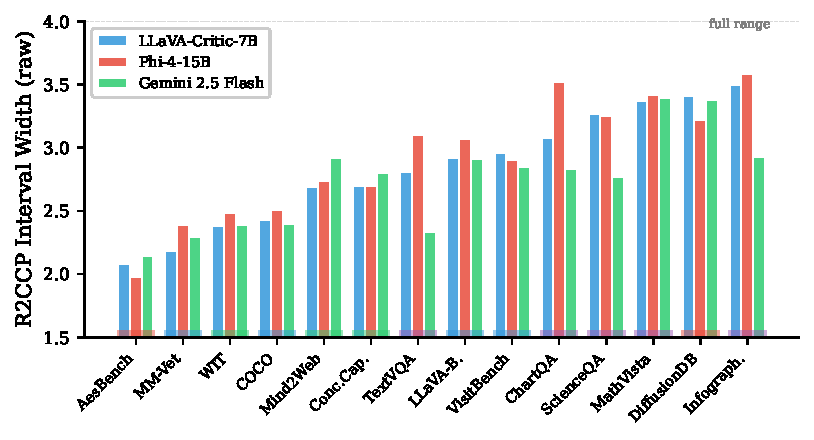
\includegraphics[width=\linewidth]{figures/task_width_comparison.pdf}
\caption{R2CCP interval width across 14 task categories for all three judges. Task-dependent uncertainty is consistent: aesthetics tasks yield tight intervals while vision-heavy tasks produce wide intervals regardless of the judge. The ordering is largely preserved across judges (Spearman $\rho = 0.82$--$0.93$).}
\label{fig:task_width}
\end{figure}

\paragraph{What drives per-dataset width?} The interval width for each dataset is determined by the interaction of three factors: (1) the judge's accuracy on that dataset (higher accuracy $\to$ narrower intervals), (2) the score distribution of the dataset (more concentrated distributions $\to$ easier prediction), and (3) the diversity of visual content within the dataset (more diverse images $\to$ harder to learn consistent nonconformity patterns). AesBench has the highest $\pm 1$ accuracy (88.3\%) and yields the narrowest intervals, while DiffusionDB has the lowest accuracy (57.2\%) and one of the widest intervals. However, ChartQA breaks this pattern---it has moderate accuracy (73.2\%) but wide intervals (3.08)---because the judge can \emph{rank} chart evaluations well but cannot assign precise scores, a phenomenon we analyze next.

\subsection{Ranking-scoring decoupling}
\label{sec:decoupling}

A striking and practically important finding emerges when comparing per-dataset Pearson correlation (ranking quality) with interval width (scoring precision). Table~\ref{tab:per_dataset} shows that ChartQA achieves the \emph{highest} Pearson correlation among all 14 datasets ($\rho = 0.507$) while producing some of the \emph{widest} intervals (width $= 3.08$, 11th out of 14 from narrowest). Conversely, WIT has low correlation ($\rho = 0.164$) but relatively narrow intervals (2.38, 3rd narrowest).

This \emph{ranking-scoring decoupling} reveals a failure mode that is \textbf{completely invisible to standard evaluation metrics}: a judge can correctly identify which answers are better or worse (high ranking correlation) while being unable to assign reliable absolute scores (wide prediction intervals). Without conformal prediction, a practitioner examining ChartQA would see the high Pearson correlation and conclude the judge is performing well---missing the fact that the judge's absolute scores are among the least reliable across all 14 task types.

\paragraph{Why does this happen?} The decoupling arises because ranking requires only monotonic relationship between judge scores and human scores (captured by correlation), while precise scoring requires accurate calibration of the score \emph{magnitude} (captured by interval width). On chart understanding tasks, the judge has enough visual comprehension to recognize that a well-structured chart interpretation is better than a poor one, producing consistent orderings. But the exact score it assigns---a 3 vs.\ a 4---is unreliable because the judge's internal calibration for chart tasks is poor.

\paragraph{Practical implications.} This finding has direct consequences for VLM judge deployment:
\begin{itemize}[leftmargin=*,itemsep=1pt,topsep=2pt]
\item For tasks where only \emph{relative ordering} matters (model selection, preference learning, reward model training), standard correlation metrics remain appropriate, and chart understanding is a strong suit for VLM judges.
\item For tasks requiring \emph{absolute quality scores} (quality thresholding, automated grading, compliance checking), wide conformal intervals reveal that the judge's point scores are unreliable, even when ranking metrics appear strong. \textbf{Pairwise comparison should be preferred over Likert scoring for such tasks.}
\item The decoupling is \emph{task-specific}: it cannot be predicted from aggregate metrics. Per-task conformal analysis is necessary to identify which tasks suffer from this phenomenon.
\end{itemize}

Gemini exhibits the decoupling most clearly (Figure~\ref{fig:decoupling}): on TextVQA, it achieves Pearson $= 0.600$ with width $= 2.33$ (tight intervals), while on Mind2Web, Pearson drops to $0.065$ but width is a similar $2.92$. High correlation does not guarantee tight intervals, and the relationship between ranking quality and scoring precision is task-dependent.

\begin{figure}[t]
\centering
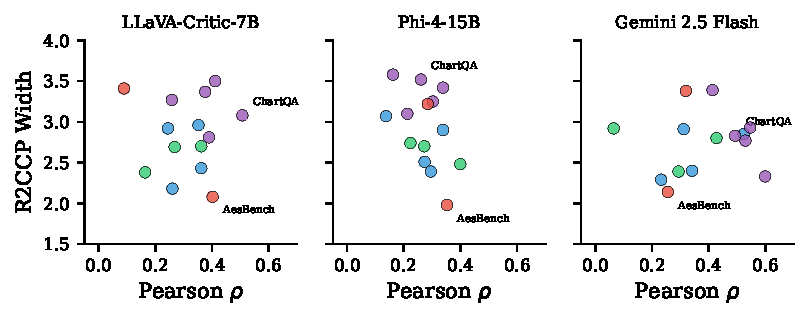
\includegraphics[width=\linewidth]{figures/ranking_scoring_decoupling.pdf}
\caption{Ranking-scoring decoupling across judges. Each point is one of 14 datasets; color indicates task category (purple=Vision-Heavy, blue=General VQA, green=Knowledge, red=Aesthetics). High Pearson correlation does not imply narrow intervals. ChartQA has the highest correlation for LLaVA-Critic but produces wide intervals, while AesBench has moderate correlation but the tightest intervals.}
\label{fig:decoupling}
\end{figure}

\subsection{Effect of ground truth quality: MLLM-Judge vs.\ Polaris}
\label{sec:polaris}

\begin{figure}[t]
\centering
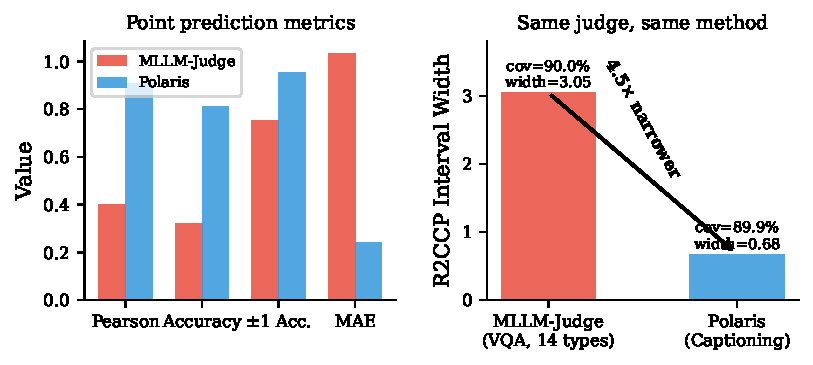
\includegraphics[width=\linewidth]{figures/polaris_comparison.pdf}
\caption{MLLM-Judge vs.\ Polaris: same judge (LLaVA-Critic-7B), same CP method (R2CCP, $\alpha=0.10$), but $4.5\times$ narrower intervals when ground truth is clean (multi-annotator) and the task is well-defined (captioning).}
\label{fig:polaris}
\end{figure}

\begin{table}[t]
\centering
\caption{Same judge (LLaVA-Critic-7B), same method (R2CCP, $\alpha=0.10$)---dramatically different results. Multi-annotator GT and well-defined task yield $4.5\times$ narrower intervals. Both achieve the target 90\% coverage.}
\label{tab:polaris}
\small
\begin{tabular}{lcc}
\toprule
& \textbf{MLLM-Judge} & \textbf{Polaris} \\
& \textbf{(VQA, 14 types)} & \textbf{(Captioning)} \\
\midrule
Samples & 5,717 & 8,726 \\
GT type & 1 annotator, integer & 3+ annotators, avg. \\
Task types & 14 diverse visual tasks & 1 task (captions) \\
\midrule
\multicolumn{3}{l}{\emph{Point prediction}} \\
Pearson $\rho$ & .402 & \textbf{.906} \\
Accuracy & 32.2\% & \textbf{80.9\%} \\
$\pm 1$ Accuracy & 75.1\% & \textbf{95.4\%} \\
MAE & 1.031 & \textbf{0.243} \\
Bias & $+0.380$ & $\mathbf{-0.062}$ \\
\midrule
\multicolumn{3}{l}{\emph{Conformal prediction (R2CCP)}} \\
R2CCP Coverage & .900 & .899 \\
\textbf{R2CCP Width} & 3.05 (61\% of range) & \textbf{0.68 (14\% of range)} \\
\bottomrule
\end{tabular}
\end{table}

Table~\ref{tab:polaris} and Figure~\ref{fig:polaris} present perhaps the most illuminating comparison in our study. Using the \emph{same} judge (LLaVA-Critic-7B) and the \emph{same} conformal method (R2CCP with $\alpha = 0.10$), we obtain dramatically different interval widths: 3.05 on MLLM-Judge (61\% of the score range) vs.\ 0.68 on Polaris (14\% of the score range)---a \textbf{$4.5\times$ reduction}. Both datasets achieve the target 90\% coverage ($0.900$ and $0.899$ respectively).

Notably, this advantage is judge-dependent: Phi-4-15B with chain-of-thought reasoning achieves only Pearson $= 0.128$ and R2CCP width $= 3.60$ on a balanced 924-sample Polaris subset---\emph{worse} than LLaVA-Critic despite being twice the size. Without reasoning mode, Phi-4 degrades further to Pearson $= 0.036$, defaulting to score 4 for 72\% of samples. This demonstrates that \textbf{model specialization matters more than model scale}: LLaVA-Critic, trained specifically for evaluation, dramatically outperforms a general-purpose reasoning model on captioning assessment.

The LLaVA-Critic result demonstrates conclusively that \textbf{interval width is driven by the evaluation task and ground truth quality, not the conformal prediction method or the judge model}. Three factors explain the 4.5$\times$ difference:

\begin{enumerate}[leftmargin=*,itemsep=1pt,topsep=2pt]
\item \textbf{Task simplicity:} Caption quality assessment is a single, well-defined task (``does this caption describe the image?'') compared to 14 diverse visual reasoning tasks spanning mathematics, chart interpretation, web navigation, and aesthetics.
\item \textbf{Annotation quality:} Multi-annotator averaged ground truth is substantially less noisy than single-annotator integer labels. Averaging across 3+ annotators smooths out individual annotator biases and disagreements. The continuous scores also provide finer-grained signal for conformal calibration.
\item \textbf{Judge accuracy:} The judge achieves Pearson $= 0.906$ on Polaris vs.\ $0.402$ on MLLM-Judge, providing conformal prediction with much stronger signal to construct tight intervals. The 80.9\% exact accuracy (vs.\ 32.2\%) means the nonconformity scores are concentrated near zero for most samples.
\end{enumerate}

\paragraph{Implications.} This finding has two important implications. First, when evaluating a new domain where the VLM judge performs well on a well-defined task with clean annotations, practitioners should expect tight, actionable conformal intervals---the method works excellently in favorable conditions. Second, the wide intervals on MLLM-Judge are not a limitation of conformal prediction but an accurate reflection of the genuine difficulty of evaluating diverse visual reasoning tasks with noisy single-annotator labels. \textbf{The intervals are wide because the task is hard, not because the method is weak.}

\subsection{Relationship to text-only LLM judges}
\label{sec:llm_comparison}

\citet{sheng2025analyzing} apply the same conformal framework to text-only LLM judges (GPT-4o mini, DeepSeek-R1-32B, Qwen2.5-72B) on summarization and reasoning benchmarks. Direct width comparisons across papers are not meaningful because multiple confounded factors differ simultaneously: judge scale (32B--72B vs.\ our 7B--15B), ground truth format (averaged from 3 annotators producing 13 fractional values vs.\ our single-annotator integers), and task difficulty (text summarization vs.\ 14 diverse visual reasoning domains).

However, our within-study comparison provides the key insight. \citet{sheng2025analyzing} use averaged multi-annotator GT scores, similar to our Polaris dataset. On Polaris (multi-annotator, well-defined captioning task), our 7B VLM judge achieves R2CCP width of 0.68---demonstrating that conformal prediction produces tight intervals when conditions are favorable. The wider intervals on MLLM-Judge (3.05) reflect the harder task and noisier annotations, not a limitation of the visual modality.

\paragraph{Key adaptation: 5-class vs.\ 13-class.} \citet{sheng2025analyzing} use 13-class interpolation for their quasi-continuous averaged GT scores. Our integer GT has only 5 discrete values, so we use 5-class direct prediction in R2CCP. This is a necessary adaptation: the 13-class interpolation would place our integer labels on only 5 of 13 class centers, wasting model capacity on unused bins. Our 5-class approach matches the ground truth granularity exactly.

\subsection{Mondrian CP: task-conditional intervals}
\label{sec:mondrian_results}

Table~\ref{tab:mondrian} presents the results of Mondrian conformal prediction, which computes separate conformal quantiles for easy, medium, and hard task groups (defined in \S\ref{sec:mondrian}). Compared to standard R2CCP (which uses a single global quantile), Mondrian CP produces substantially different interval properties across difficulty groups.

\begin{table}[t]
\centering
\caption{Mondrian CP vs.\ standard R2CCP (LLaVA-Critic-7B, boundary-adjusted, 10 seeds). Mondrian narrows easy-task intervals by 16.6\% while improving hard-task coverage from 96.7\% to 98.2\%.}
\label{tab:mondrian}
\small
\begin{tabular}{lcccc}
\toprule
& \multicolumn{2}{c}{\textbf{Standard R2CCP}} & \multicolumn{2}{c}{\textbf{Mondrian R2CCP}} \\
\cmidrule(lr){2-3} \cmidrule(lr){4-5}
\textbf{Group} & \textbf{Cov.} & \textbf{Width} & \textbf{Cov.} & \textbf{Width} \\
\midrule
Easy & 99.0\% & 3.55 & 97.5\% & \textbf{2.96} ($-$16.6\%) \\
Medium & 99.1\% & 3.60 & 98.7\% & \textbf{3.49} ($-$3.1\%) \\
Hard & 96.7\% & 3.63 & \textbf{98.2\%} & 3.78 ($+$4.1\%) \\
\midrule
Overall & 98.1\% & 3.60 & 98.2\% & \textbf{3.47} ($-$3.6\%) \\
\bottomrule
\end{tabular}
\end{table}

\paragraph{Key findings.} Mondrian CP achieves a favorable tradeoff: (1)~easy tasks (AesBench, MM-Vet, WIT, COCO) receive \textbf{16.6\% narrower intervals} (2.96 vs.\ 3.55), making the intervals substantially more informative for decision-making; (2)~hard tasks (ScienceQA, MathVista, DiffusionDB, InfographicsVQA) receive \textbf{improved coverage} (98.2\% vs.\ 96.7\%), providing stronger guarantees where they are most needed; (3)~overall width decreases by 3.6\% (3.47 vs.\ 3.60) while maintaining equivalent overall coverage (98.2\% vs.\ 98.1\%).

The intuition is straightforward: standard CP computes a global quantile that must be large enough to cover the hardest tasks, resulting in unnecessarily wide intervals for easy tasks. Mondrian CP allows each group to have its own quantile, removing this cross-contamination. The slight coverage decrease for easy tasks (99.0\% $\to$ 97.5\%) is by design---the standard CP was substantially over-covering, and Mondrian CP brings coverage closer to the $1 - \alpha + \text{adjustment}$ target while reclaiming the excess width.

This is, to our knowledge, the \textbf{first application of Mondrian conformal prediction to VLM judge evaluation}. It demonstrates that task-conditional calibration is both feasible and beneficial when evaluation tasks have known difficulty structure.

\subsection{CP-Reliability Diagnostic}
\label{sec:rsg_results}

\begin{table}[t]
\centering
\caption{CP-Reliability Diagnostic: Ranking-Scoring Gap (RSG) for all 3 judges. Positive RSG = judge ranks well but can't score precisely (use pairwise comparison). Negative RSG = intervals are more informative than ranking suggests. Top-3 RSG datasets highlighted.}
\label{tab:rsg}
\small
\begin{tabular}{lcccccc}
\toprule
& \multicolumn{2}{c}{\textbf{LLaVA}} & \multicolumn{2}{c}{\textbf{Phi-4}} & \multicolumn{2}{c}{\textbf{Gemini}} \\
\cmidrule(lr){2-3} \cmidrule(lr){4-5} \cmidrule(lr){6-7}
\textbf{Dataset} & $\rho$ & RSG & $\rho$ & RSG & $\rho$ & RSG \\
\midrule
Infograph. & .411 & \textbf{+.287} & .162 & +.058 & .547 & \textbf{+.281} \\
ChartQA & .507 & \textbf{+.276} & .261 & +.141 & .494 & \textbf{+.201} \\
MathVista & .376 & \textbf{+.219} & .339 & +.194 & .414 & \textbf{+.262} \\
VisitBench & .352 & +.091 & .339 & +.064 & .524 & +.235 \\
ScienceQA & .258 & +.075 & .304 & +.115 & .530 & +.223 \\
TextVQA & .389 & +.092 & .213 & $-$.012 & .600 & +.183 \\
\midrule
WIT & .164 & $-$.242 & .400 & +.021 & .294 & $-$.109 \\
MM-Vet & .260 & $-$.195 & .296 & $-$.108 & .233 & $-$.194 \\
AesBench & .402 & $-$.077 & .353 & $-$.153 & .256 & $-$.208 \\
\bottomrule
\end{tabular}
\end{table}

Table~\ref{tab:rsg} presents the Ranking-Scoring Gap diagnostic across all three judges. The RSG consistently identifies the same problematic datasets across judges:

\paragraph{High-RSG datasets (ranking $\gg$ scoring).} InfographicsVQA ($+0.287$), ChartQA ($+0.276$), and MathVista ($+0.219$) consistently have the highest RSG across all three judges. These are Vision-Heavy tasks where the judge can detect quality differences between answers (producing good rankings) but cannot calibrate its confidence to produce tight intervals. For these tasks, \textbf{practitioners should prefer pairwise comparison over Likert scoring}.

\paragraph{Negative-RSG datasets (scoring $>$ ranking).} WIT ($-0.242$), MM-Vet ($-0.195$), and AesBench ($-0.077$) have negative RSG: the intervals are more informative than the Pearson correlation would suggest. This occurs when the judge produces well-calibrated score distributions (low nonconformity) even though its point predictions have moderate correlation with ground truth. For these tasks, absolute Likert scoring is viable.

\paragraph{Cross-judge consistency.} The top-3 RSG datasets (InfographicsVQA, ChartQA, MathVista) are the same for LLaVA-Critic and Gemini, and 2 of 3 overlap for Phi-4. This confirms that the ranking-scoring decoupling is a property of the task, not the judge---Vision-Heavy tasks involving structured visual reasoning consistently exhibit this gap.

\subsection{Multi-judge feature fusion}
\label{sec:multijudge}

A natural question is whether combining logprob features from multiple judges produces better conformal intervals than using a single judge. We concatenate the 5-dimensional S2 features from each judge into joint feature vectors and train R2CCP on the combined features.

\begin{table}[t]
\centering
\caption{Multi-judge feature fusion (R2CCP, 10 seeds). Combining judges does NOT outperform the best single judge (Gemini). Logprob quality $>$ quantity.}
\label{tab:multijudge}
\small
\begin{tabular}{lrccc}
\toprule
\textbf{Configuration} & \textbf{Feat.} & \textbf{Cov.} & \textbf{Width} & \textbf{Width} \\
& & \textbf{(raw)} & \textbf{(raw)} & \textbf{(adj.)} \\
\midrule
Gemini only & 5 & .898 & \textbf{2.85} & \textbf{3.41} \\
LLaVA + Gemini & 10 & .901 & 3.02 & 3.51 \\
LLaVA only & 5 & .900 & 3.05 & 3.60 \\
Multi-Judge (all 3) & 15 & .905 & 3.14 & 3.56 \\
LLaVA + Phi-4 & 10 & .903 & 3.18 & 3.62 \\
Phi-4 only & 5 & .891 & 3.13 & 3.70 \\
\bottomrule
\end{tabular}
\end{table}

Table~\ref{tab:multijudge} reveals a clear \textbf{negative result}: combining all three judges' logprobs (15 features) produces \emph{wider} intervals (3.14) than Gemini alone (2.85)---a 10\% degradation. Even the best combination (LLaVA + Gemini, 10 features) at 3.02 is wider than Gemini alone. Adding Phi-4's features to any combination hurts performance.

\paragraph{Why fusion fails.} R2CCP's neural network must learn a mapping from features to nonconformity scores. With 15 features but only ${\sim}2{,}850$ calibration samples, the model faces a higher-dimensional learning problem without proportionally more signal. The additional features from weaker judges (Phi-4 Pearson $= 0.303$, LLaVA $= 0.402$) introduce noise that dilutes the strong signal from Gemini ($= 0.459$). The neural network cannot effectively learn to weight the better judge's features more heavily with limited calibration data.

\paragraph{Practical implication.} \textbf{For conformal prediction with VLM judges, logprob quality matters more than quantity.} Practitioners should invest in one high-quality judge with informative logprobs rather than ensembling multiple mediocre judges. This is particularly relevant given the cost considerations: running three judges (two requiring GPU resources, one requiring API calls) provides no benefit over using Gemini alone.

% ============================================================================
\section{Analysis}
\label{sec:analysis}

\subsection{Conformal prediction as a safety net: recovering judge errors}
\label{sec:cp_value}

\begin{figure}[t]
\centering
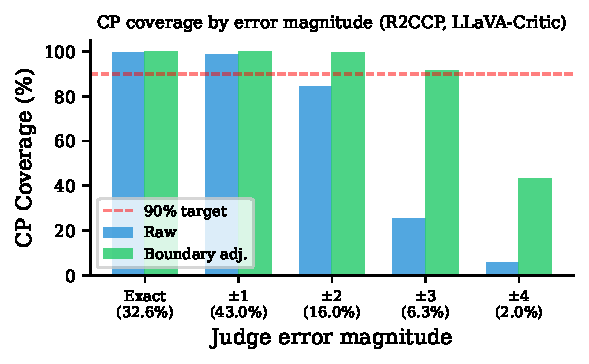
\includegraphics[width=0.75\linewidth]{figures/error_bin_coverage.pdf}
\caption{CP coverage by error magnitude (R2CCP, LLaVA-Critic-7B). Boundary adjustment is critical: for $\pm 2$ errors, raw coverage is only 84\% but adjusted coverage reaches 99\%. Overall, CP with boundary adjustment recovers 97.8\% of all judge errors.}
\label{fig:error_bins}
\end{figure}

\begin{table}[t]
\centering
\caption{CP coverage by error magnitude (R2CCP, LLaVA-Critic-7B, 10 seeds). CP with boundary adjustment recovers 97.8\% of all judge errors. For the 59\% of wrong predictions with $\pm 1$--$\pm 2$ errors, adjusted coverage exceeds 99\%.}
\label{tab:error_bins}
\small
\begin{tabular}{lrcccc}
\toprule
\textbf{Error} & \textbf{\%} & \textbf{Cov.} & \textbf{Cov.} & \textbf{Width} & \textbf{Width} \\
$|y_0 - y|$ & \textbf{samp.} & \textbf{(raw)} & \textbf{(adj.)} & \textbf{(raw)} & \textbf{(adj.)} \\
\midrule
0 (exact) & 32.6\% & 99.8\% & 100\% & 2.98 & 3.55 \\
$\pm 1$ & 43.0\% & 98.7\% & 99.9\% & 3.08 & 3.63 \\
$\pm 2$ & 16.0\% & 84.3\% & 99.4\% & 3.12 & 3.65 \\
$\pm 3$ & 6.3\% & 25.4\% & 91.5\% & 3.05 & 3.61 \\
$\pm 4$ & 2.0\% & 5.7\% & 43.3\% & 2.89 & 3.42 \\
\midrule
\multicolumn{6}{l}{\emph{Overall: 97.8\% of 1,927 errors recovered (seed=1)}} \\
\bottomrule
\end{tabular}
\end{table}

The practical value of conformal prediction becomes clearest when examining its behavior on judge errors (Table~\ref{tab:error_bins}, Figure~\ref{fig:error_bins}). We stratify CP coverage by the magnitude of the judge's error.

\paragraph{CP is most valuable when the judge is wrong.} For $\pm 1$ errors (43\% of all samples), boundary-adjusted coverage reaches 99.9\%---virtually perfect. Even for $\pm 2$ errors (16\% of samples), coverage is 99.4\%. Only for the most extreme errors ($\pm 3$ and $\pm 4$, comprising 8.3\% of samples) does coverage drop significantly. Overall, of 1,927 judge errors in a single test split (seed=1), conformal intervals with boundary adjustment contain the true human score for 1,885 of them---a \textbf{97.8\% recovery rate}. Only 42 errors out of 1,927 are not covered.

\paragraph{What are the unrecovered errors?} The 42 unrecovered errors are predominantly extreme cases where the judge predicts a score of 4 or 5 but the human ground truth is 1. These are instances where the judge is \emph{maximally} wrong---overscoring a terrible answer by 3--4 points. The conformal interval, centered near the judge's predicted score, simply cannot stretch far enough to reach the true score at the opposite end of the scale. These cases represent fundamental judge failures that no post-hoc calibration method can fully address.

\paragraph{Comparison across judges.} Table~\ref{tab:error_bins_all} shows the error-bin analysis for all three judges. The recovery pattern is consistent: $>$96\% of $\pm 1$--$\pm 2$ errors are covered after boundary adjustment across all judges. Gemini achieves notably higher raw coverage for $\pm 3$ errors (53.7\% vs.\ 25.4\% for LLaVA-Critic) because Gemini's narrower but better-centered intervals are more likely to extend to the true score even for larger errors.

\begin{table}[t]
\centering
\caption{CP coverage (adjusted) by error magnitude across judges. All judges achieve $>$99\% recovery for $\pm 1$ and $\pm 2$ errors.}
\label{tab:error_bins_all}
\small
\begin{tabular}{lccc}
\toprule
\textbf{Error} & \textbf{LLaVA} & \textbf{Phi-4} & \textbf{Gemini} \\
\midrule
$\pm 1$ adj.\ cov. & 99.9\% & 99.9\% & 99.8\% \\
$\pm 2$ adj.\ cov. & 99.4\% & 99.5\% & 99.0\% \\
$\pm 3$ adj.\ cov. & 91.5\% & 86.3\% & \textbf{96.2\%} \\
$\pm 4$ adj.\ cov. & 43.3\% & 67.4\% & \textbf{68.8\%} \\
\bottomrule
\end{tabular}
\end{table}

\subsection{Boundary adjustment is disproportionately important for discrete scales}
\label{sec:boundary_analysis}

Boundary adjustment has a dramatically larger effect in our setting compared to \citet{sheng2025analyzing}'s text-only experiments. On MLLM-Judge, adjustment increases CHR coverage from 88.0\% to 96.5\% (an 8.5 percentage point gain) and R2CCP from 90.0\% to 98.1\% (an 8.1 point gain). In contrast, on their SummEval with quasi-continuous GT, the typical gain is 2--5 percentage points.

This disparity arises from a fundamental difference in ground truth granularity. Their GT uses 13 fractional values (averages of 3 annotators on a Likert scale), making it quasi-continuous---a continuous interval endpoint is likely to already cover the nearest fractional GT value. Our GT uses only 5 integer values, meaning continuous interval endpoints frequently fall between integers (e.g., an interval $[2.3, 4.7]$ that misses GT$=$2 is expanded to $[2, 4]$ which covers it). This finding has a practical implication: \textbf{boundary adjustment is essential for VLM judge applications where ground truth is discrete}, and researchers should always report both raw and adjusted metrics.

\subsection{Conditional coverage by ground truth score}
\label{sec:conditional}

While conformal prediction guarantees marginal coverage (averaged over all test samples), conditional coverage---the coverage for specific subgroups---can vary. Table~\ref{tab:conditional} stratifies coverage by ground truth score level.

\begin{table}[t]
\centering
\caption{Conditional coverage by GT score level (R2CCP, LLaVA-Critic-7B, seed=1). GT=1 is the weakest spot due to severe judge overscoring. All other GT levels achieve $\geq$99\% adjusted coverage.}
\label{tab:conditional}
\small
\begin{tabular}{lrccccc}
\toprule
\textbf{GT} & \textbf{N} & \textbf{Cov.} & \textbf{Cov.} & \textbf{Width} & \textbf{Width} & \textbf{Judge} \\
& & \textbf{(raw)} & \textbf{(adj.)} & \textbf{(raw)} & \textbf{(adj.)} & \textbf{Bias} \\
\midrule
GT$=$1 & 334 & 53.0\% & \textbf{88.9\%} & 3.14 & 3.75 & $+1.67$ \\
GT$=$2 & 360 & 86.9\% & 100\% & 3.18 & 3.79 & $+1.13$ \\
GT$=$3 & 637 & 99.7\% & 100\% & 3.09 & 3.75 & $+0.77$ \\
GT$=$4 & 880 & 98.2\% & 100\% & 2.99 & 3.65 & $+0.11$ \\
GT$=$5 & 648 & 92.4\% & 99.2\% & 2.92 & 3.58 & $-0.80$ \\
\bottomrule
\end{tabular}
\end{table}

\paragraph{GT=1 is the systematic weak spot.} Coverage drops to only 88.9\% after boundary adjustment for GT$=$1 (the lowest quality answers), well below the 90\% target. This is the \emph{only} GT level where coverage falls below target. The cause is directly linked to judge bias: all three judges substantially overscore bad answers ($+1.67$ mean bias for GT$=$1), pushing the prediction interval center far above 1. Even with boundary adjustment expanding the interval downward, the interval cannot compensate for a mean offset of $+1.67$ score points.

This pattern holds across all three judges and has a concrete practical implication: \textbf{practitioners should exercise particular caution when VLM judges evaluate clearly poor answers}. The conformal interval may fail to signal the severity of quality problems when the judge confidently assigns a middling score to a genuinely bad answer.

\paragraph{Coverage stratified by dataset.} We also verify that the marginal coverage guarantee holds across all 14 datasets individually. After boundary adjustment, all datasets achieve $\geq$96\% coverage, with the lowest being MathVista (96.0\%) and the highest being LLaVA-Bench and Conceptual Captions (100\%). The guarantee is robust even on the hardest vision-heavy tasks where judge accuracy is lowest.

\subsection{Interval informativeness}
\label{sec:informativeness}

Not all prediction intervals are equally useful for decision-making. We categorize boundary-adjusted intervals by their practical utility:

\begin{itemize}[leftmargin=*,itemsep=1pt,topsep=2pt]
\item \textbf{Decisive} (width $\leq 2$): Narrows to 2--3 possible scores. Directly actionable for quality decisions.
\item \textbf{Moderate} (width 2--3): Provides some discrimination, covering 3--4 scores. Useful for flagging high-confidence vs.\ uncertain evaluations.
\item \textbf{Uninformative} (width $> 3$): Nearly full range ($>$75\% of scores). Provides minimal additional value beyond knowing the score is somewhere in $\{1, \ldots, 5\}$.
\end{itemize}

\paragraph{MLLM-Judge results.} On MLLM-Judge, 0.5\% of intervals are decisive, 30.7\% are moderate, and 68.8\% are uninformative. The ~31\% moderate intervals provide genuine actionable information. By task category: Aesthetics/AI produces 37.7\% moderate intervals (the most informative), Vision-Heavy 31.8\%, Knowledge/Web 30.8\%, and General VQA 25.9\% (the least informative outside the uninformative category).

\paragraph{Polaris results.} The picture changes dramatically on Polaris: with average width 0.68 (less than 1 score point), the vast majority of intervals are decisive. This demonstrates that the conformal framework produces highly informative uncertainty estimates when conditions are favorable, and the high uninformative fraction on MLLM-Judge reflects the genuine difficulty of the evaluation task rather than a limitation of the approach.

\subsection{Midpoint analysis}
\label{sec:midpoint}

Following \citet{sheng2025analyzing}, we evaluate whether the midpoint of the R2CCP prediction interval provides a better score estimate than the raw judge score.

\begin{table}[t]
\centering
\caption{Midpoint of R2CCP interval vs.\ raw judge score (LLaVA-Critic-7B, seed=1). Unlike Sheng et al.'s finding for text-only judges, midpoint does not consistently improve over the raw score for VLM judges.}
\label{tab:midpoint}
\small
\begin{tabular}{lccc}
\toprule
\textbf{Metric} & \textbf{Raw Score} & \textbf{Midpoint (raw)} & \textbf{Midpoint (adj.)} \\
\midrule
Pearson $\rho$ & \textbf{.412} & .396 & .277 \\
Spearman $\rho_s$ & \textbf{.367} & .359 & .272 \\
MAE & 1.022 & \textbf{0.992} & 1.056 \\
Accuracy & \textbf{32.6\%} & --- & 28.1\% \\
\bottomrule
\end{tabular}
\end{table}

Table~\ref{tab:midpoint} shows that the raw-interval midpoint achieves slightly lower MAE (0.992 vs.\ 1.022) but lower correlation ($\rho = 0.396$ vs.\ $0.412$). The boundary-adjusted midpoint performs worse on all metrics. \textbf{Unlike \citet{sheng2025analyzing}'s finding for text-only judges, the midpoint does not consistently improve over the raw VLM judge score.}

The explanation is straightforward: our intervals are wide (average 3.05), so the midpoint regresses strongly toward the center of the scale (${\sim}3.0$). In \citet{sheng2025analyzing}'s setting, intervals are narrower (0.6--2.5), so the midpoint stays close to the judge's original prediction while benefiting from the interval's centering effect. When intervals span most of the scale, the midpoint loses the discriminative signal present in the raw score.

\subsection{Gemini per-dataset advantages}
\label{sec:gemini_advantages}

Gemini produces narrower intervals than both open-source judges on 10 of 14 datasets (Table~\ref{tab:all_judges_per_dataset} in Appendix~\ref{app:per_dataset}). The largest improvements are on Vision-Heavy tasks: TextVQA ($-0.48$ vs.\ LLaVA-Critic), ScienceQA ($-0.50$), InfographicsVQA ($-0.57$), and ChartQA ($-0.25$). These are precisely the tasks where structured visual understanding matters most, suggesting that Gemini's larger scale and training provide genuine advantages in parsing charts, diagrams, and text in images. The datasets where Gemini does \emph{not} improve are Knowledge/Web (Mind2Web: $+0.23$) and Aesthetics (DiffusionDB: $-0.03$), where the task relies more on subjective judgment than visual parsing ability.

% ============================================================================
\section{Discussion}
\label{sec:discussion}

\paragraph{Practical guidance for VLM judge deployment.}
Our results offer concrete, actionable guidance for practitioners deploying VLM judges:

\begin{enumerate}[leftmargin=*,itemsep=2pt,topsep=2pt]
\item \textbf{Always run conformal prediction alongside VLM judge evaluation.} The cost is minimal (one forward pass for logprob extraction plus lightweight CP calibration) and the benefits are substantial: per-instance uncertainty estimates with provable coverage guarantees, especially for the ${\sim}59\%$ of errors within $\pm 1$--$\pm 2$ points where boundary-adjusted coverage exceeds 99\%.

\item \textbf{Use interval width as a per-task reliability indicator.} A judge with 33\% accuracy on aesthetics tasks is far more trustworthy (width 2.1) than a judge with 33\% accuracy on math reasoning (width 3.4). Aggregate accuracy numbers are misleading without task-specific uncertainty quantification.

\item \textbf{Prefer pairwise comparison over Likert scoring for tasks exhibiting ranking-scoring decoupling.} For chart understanding, the judge ranks well (Pearson $= 0.507$) but scores unreliably (width $= 3.08$). Using pairwise comparisons preserves the ranking ability while avoiding the unreliable absolute scores.

\item \textbf{Invest in annotation quality.} The $4.5\times$ narrower intervals on Polaris (multi-annotator) vs.\ MLLM-Judge (single annotator) suggest that improving ground truth quality may be more impactful than scaling judge models or developing better conformal methods.

\item \textbf{Use R2CCP with boundary adjustment as the default configuration.} R2CCP achieves exact 90\% coverage with the best width among well-calibrated methods, and boundary adjustment is essential for discrete rating scales.

\item \textbf{Be cautious about GT=1 predictions.} All judges overscore bad answers, causing conditional coverage to drop below 90\% for the lowest quality bin. Consider flagging evaluations where the judge assigns a low score with high uncertainty.
\end{enumerate}

\paragraph{What drives interval width?}
Our experiments identify three factors that determine conformal interval width, in decreasing order of importance: (1)~\textbf{ground truth quality}---the $4.5\times$ improvement from MLLM-Judge to Polaris demonstrates that multi-annotator averaged labels produce dramatically tighter intervals; (2)~\textbf{task difficulty}---within MLLM-Judge, width varies 70\% across 14 task types even with the same judge and annotation format; (3)~\textbf{judge quality}---Gemini's higher Pearson correlation ($0.459$) produces 7\% narrower intervals than LLaVA-Critic ($0.402$). The conformal method and number of features matter much less: R2CCP outperforms Naive CP by only 13\%, and adding more judge features actually hurts (multi-judge fusion is 10\% worse than the best single judge). These findings suggest that practitioners should prioritize annotation quality and task-specific evaluation over scaling conformal methods or ensembling judges.

\paragraph{Connection to VLM hallucination and reliability research.}
Our findings connect to broader concerns about VLM reliability. The task-dependent uncertainty we observe---wider intervals on chart understanding, math reasoning, and AI-generated images---aligns with known failure modes of VLMs: visual hallucination~\citep{li2024vlrewardbench}, poor compositional understanding, and unreliable spatial reasoning. Conformal prediction provides a principled, quantitative framework for measuring these reliability differences across task types, complementing the qualitative error analyses in existing VLM benchmarks.

The positive bias we observe (all judges overscoring bad answers) echoes the ``sycophancy'' phenomenon documented in LLM judges~\citep{zheng2023judging}: models prefer to give positive evaluations, potentially because their training data is biased toward positive feedback or because chain-of-thought reasoning leads them to find positive aspects even in poor answers. Conformal prediction cannot correct this bias, but the wide intervals it produces for biased predictions serve as a valuable warning signal.

\paragraph{Limitations.}
Our study has several limitations that suggest directions for future work:

\begin{enumerate}[leftmargin=*,itemsep=1pt,topsep=2pt]
\item \textbf{Judge scale:} Our VLM judges (7B--15B open-source) are smaller than the 32B--72B models used by \citet{sheng2025analyzing}. A controlled comparison using the same-scale models across modalities (e.g., Qwen2.5-72B for text vs.\ Qwen2.5-VL-72B for vision) would isolate the effect of the visual modality on conformal prediction performance.

\item \textbf{Feature engineering:} We use only Signal 2 (score-token logprobs, 5 dimensions). We explored visual grounding features (CLIPScore of image-answer similarity) as an additional signal, but found no correlation with judge error (Pearson $= -0.017$, $p = 0.73$)---CLIPScore measures whether the answer is \emph{about} the image, not whether it is \emph{correct} about the image. Generation-level token entropy and attention-based features remain unexplored directions.

\item \textbf{Number of seeds:} We use 10 random seeds vs.\ 30 in \citet{sheng2025analyzing}. However, our substantially larger dataset (5,717 vs.\ $\sim$200--1,600 samples) provides comparable or greater statistical power per seed.

\item \textbf{Single-annotator ground truth:} The MLLM-Judge benchmark uses single-annotator labels, which may conflate genuine judge error with annotator disagreement. Multi-annotator ground truth (as in Polaris) would provide a cleaner signal, and the dramatic improvement we observe on Polaris supports this hypothesis.

\item \textbf{Conditional coverage:} Conformal prediction guarantees only marginal coverage. Our analysis reveals that conditional coverage by GT score varies substantially (88.9\% for GT$=$1 vs.\ 100\% for GT$=$3), suggesting that methods for improving conditional coverage~\citep{angelopoulos2022conformal} may be valuable in this setting.

\item \textbf{Evaluation scope:} We focus on single-answer Likert scoring. Extending to pairwise preference evaluation, multi-aspect scoring (e.g., separate scores for accuracy, relevance, fluency), or open-ended evaluation remains future work.
\end{enumerate}

% ============================================================================
\section{Conclusion}
\label{sec:conclusion}

We present the first systematic study of conformal prediction for VLM-as-a-Judge, evaluating 8 conformal methods across 3 VLM judges (LLaVA-Critic-7B, Phi-4-reasoning-15B, Gemini 2.5 Flash) and 14,443 multimodal evaluation instances across 2 benchmarks. Our analysis reveals several findings with direct implications for VLM judge deployment:

\begin{enumerate}[leftmargin=*,itemsep=2pt,topsep=2pt]
\item \textbf{Evaluation uncertainty is strongly task-dependent}, varying by up to 70\% across 14 visual task categories. This pattern is consistent across all three judges (Spearman $\rho = 0.82$--$0.93$), indicating it is a property of the tasks themselves.

\item \textbf{A ranking-scoring decoupling exists}, formalized through our Ranking-Scoring Gap diagnostic, where judges rank responses accurately while producing unreliable absolute scores. InfographicsVQA, ChartQA, and MathVista consistently exhibit the highest RSG across all judges.

\item \textbf{Mondrian conformal prediction} conditioned on task difficulty produces 16.6\% narrower intervals for easy tasks while improving coverage for hard tasks---the first application of task-conditional CP to VLM evaluation.

\item \textbf{Multi-judge feature fusion does not outperform the best single judge}---logprob quality matters more than quantity. Practitioners should invest in one good judge rather than ensembling multiple mediocre ones.

\item \textbf{Interval width reflects task difficulty and annotation quality:} the same judge and method produce $4.5\times$ narrower intervals (0.68 vs.\ 3.05) when ground truth is clean and the task is well-defined.

\item \textbf{R2CCP is the recommended method} for VLM judge calibration, achieving exact 90\% coverage. CQR-based methods fail in this weak-feature regime.
\end{enumerate}

These findings establish conformal prediction as essential infrastructure for trustworthy deployment of VLM judges, providing practitioners with the first uncertainty-aware reliability map for multimodal evaluation. We hope this work encourages the adoption of uncertainty quantification as a standard component of VLM-as-a-Judge pipelines.

% ============================================================================
\section*{Reproducibility statement}
All experiments use publicly available models (LLaVA-Critic-7B, Phi-4-reasoning-vision-15B) and datasets (MLLM-as-a-Judge, Polaris). Gemini 2.5 Flash is accessed via the Google Vertex AI API. We will release our complete code, including inference scripts, feature extraction pipeline, conformal prediction runners, and all result CSVs upon acceptance. Results are reported across 10 random seeds with mean $\pm$ standard deviation. All conformal prediction methods use publicly available implementations (R2CCP from the authors' wheel, MAPIE v0.8.6 for CQR variants, custom implementations following published algorithms for CHR, LVD, Boosted methods, and OrdinalAPS). Hardware: 2$\times$ RTX 6000 Ada GPUs (48GB each) for open-source model inference.

\section*{Ethics statement}
Our work analyzes the reliability of automated VLM evaluators and does not introduce new evaluation capabilities---it quantifies the uncertainty of existing ones. We note several ethical considerations: (1) Conformal prediction guarantees are marginal (averaged over the calibration/test split) rather than conditional, and should not be over-interpreted as individual-instance confidence. (2) Biased human annotations in the calibration set propagate to biased prediction intervals---conformal prediction cannot correct for systematic annotator bias. (3) The positive bias we observe (judges overscoring bad answers) may mask quality problems in deployed AI systems if interval information is ignored. We encourage practitioners to use conformal intervals as a complement to, not a replacement for, careful human evaluation in high-stakes settings.


\bibliography{references}
\bibliographystyle{colm2026_conference}

\end{document}
